\documentclass[conference]{IEEEtran}
\IEEEoverridecommandlockouts
\usepackage{cite}
\usepackage{amsmath,amssymb,amsfonts}
\usepackage{algorithmic}
\usepackage{graphicx}
\usepackage{textcomp}
\usepackage{xcolor}
\usepackage{booktabs}
\usepackage{url}
\def\BibTeX{{\rm B\kern-.05em{\sc i\kern-.025em b}\kern-.08em
    T\kern-.1667em\lower.7ex\hbox{E}\kern-.125emX}}

\begin{document}

\title{CALM: Calibrated, Order-Invariant, Label-Efficient Medical Question Answering with Small Language Models on a Two-GPU Budget}

\author{
\IEEEauthorblockN{Sabarna Saha}
\IEEEauthorblockA{\textit{Dept. of Power Engineering} \\
\textit{Jadavpur University}\\
Kolkata, India \\
sabarna.saha1308@gmail.com}
\and
\IEEEauthorblockN{Ankush Sil Sarma}
\IEEEauthorblockA{\textit{AI Engineer} \\
\textit{ZS Associates}\\
Pune, India \\
ankushsil17@gmail.com}
\and
\IEEEauthorblockN{Pawan Kumar Singh}
\IEEEauthorblockA{\textit{Dept. of Information Technology} \\
\textit{Jadavpur University}\\
Kolkata, India \\
pawansingh.ju@gmail.com}
}

\maketitle

\begin{abstract}
Our budget is small on purpose: two Kaggle T4 GPUs with 16\,GB each, a few thousand labels, and 4-bit adapters. Inside it we build CALM (Calibrated, Abstention-aware, Label-efficient Medical QA). A small student is adapted with QLoRA, calibrated with a single temperature, and given a confidence-based abstention rule. A Qwen2.5-7B student trained on 2{,}000 MedQA-USMLE labels scores 0.633 (95\% CI [0.606, 0.660]); one temperature parameter cuts expected calibration error from 0.086 to 0.026, and the most confident half of the test set is answered at 80.8\% accuracy. We then ask how to push accuracy without more labels or training. A training-free order-invariant readout---averaging the calibrated prediction over the four cyclic option orderings---raises test accuracy to 0.655 (paired $+0.022$, 95\% CI $[+0.006,+0.038]$) and lowers area-under-risk--coverage, at four forward passes and no decoding. Notably, removing the option-ID prior alone does nothing here, because that prior is near-uniform: the gain is reduction of order-dependent variance, not letter debiasing. A confidence-gated reflective router, which sends only the least-confident items to a reasoning pass, adds a small but significant gain at roughly two extra decoded tokens per question, whereas a dedicated trained reflect adapter does not beat the base student's own reasoning. We are equally candid about what failed: a teacher-guided self-distillation stage never improves validation accuracy, and five-sample self-consistency loses to a single calibrated pass. The recipe that remains is short: a stronger base, light supervised adaptation, temperature calibration, abstention, and an order-invariant readout.
\end{abstract}

\begin{IEEEkeywords}
medical question answering, calibration, selective prediction, selection bias, adaptive computation, parameter-efficient fine-tuning, resource-constrained learning
\end{IEEEkeywords}

\section{Introduction}
One MedQA-USMLE question can fold a patient's age, a handful of symptoms, a lab panel, and a treatment history into a single stem, then ask for one of four plausible options \cite{medqa}. Large models handle this well. GPT-4 lands in the high eighties \cite{gpt4med} and Med-PaLM~2 in the mid eighties \cite{medpalm}. Even compact 7--8B specialists such as Meerkat \cite{meerkat} and MedMobile \cite{medmobile} clear 60\%, but only after training on the full benchmark with a great deal of reasoning data. None of that fits a lab whose entire compute is a Kaggle session with two 16\,GB T4s.

We chose to stay inside that limit. A leaderboard spot was never the goal; a working system on a fixed, small budget was. A useful medical model should also know when it is out of its depth. Accuracy on its own hides two things a clinician would ask about first: whether the confidence means anything, and whether the model can decline a question it is likely to miss \cite{trustsurvey}. CALM is built around those two questions. It tracks accuracy, calibration, and abstention quality together, and treats the last two as first-class.

We start from a supervised QLoRA student, then ask what cheap, post-hoc additions actually help. Two do. A single calibration temperature makes confidence meaningful and powers a working abstention rule. And a training-free readout that averages the prediction over the four cyclic orderings of the options removes an order-dependent wobble we did not expect to matter, lifting accuracy by more than two points. Two other ideas help only a little or not at all, and we say so plainly: routing the least-confident questions to a reasoning pass buys a small, significant gain, but a teacher-guided self-distillation stage and a dedicated reasoning adapter do not.

Our contributions are as follows.
\begin{itemize}
\item \textbf{CALM}, a reproducible study of small-LM medical QA under a strict 2$\times$T4, few-thousand-label budget, covering 3B and 7B students with 4-bit QLoRA.
\item A \textbf{calibration-and-abstention layer} that reduces test ECE to 0.026 for the 7B student and supports a risk--coverage analysis in which the most confident 50\% of test items are answered at 0.808 accuracy.
\item A \textbf{training-free order-invariant readout} that marginalizes over the four cyclic option orderings, raising test accuracy from 0.633 to 0.655 (paired 95\% CI $[+0.006,+0.038]$) and lowering AURC at four forward passes and no decoding. We show the gain is \emph{not} option-ID debiasing---that prior is near-uniform and removing it (PriDe) does nothing---but reduction of order-dependent variance.
\item A \textbf{reflective routing} study of adaptive compute: routing only the least-confident $\approx$2\% of items to a reasoning pass gives a small significant gain at $\approx$2 extra decoded tokens per question, while a trained reflect adapter does not beat the base student's own reasoning (a negative result).
\item \textbf{Two further negative results}: the teacher-guided self-distillation stage does not beat supervised adaptation at this budget, and self-consistency reasoning underperforms a single calibrated pass while costing far more decoding.
\end{itemize}

\section{Related Work}
\textbf{Medical QA with language models.} Jin et al. built MedQA from licensing exams and made the task a standard probe \cite{medqa}. Large general models answer it well with prompting alone \cite{gpt4med,medpalm}, and a line of compact specialists---Meerkat \cite{meerkat}, MedMobile \cite{medmobile}, and the HuatuoGPT-o1 reasoning models \cite{huatuo}---has narrowed the gap with curated reasoning traces. We use HuatuoGPT-o1-7B as a teacher but spend nothing close to their training budget.

\textbf{Distillation and self-training.} Hinton et al. framed soft-target transfer \cite{hinton}; STaR \cite{star} and self-consistency \cite{selfconsistency} showed generated reasoning can bootstrap smaller models. Confidence-thresholded pseudo-labeling is the workhorse of semi-supervised learning \cite{pseudolabel}. CALM combines these with explicit agreement gates; our measurements then clarify when the marginal labels help and when they do not.

\textbf{Parameter-efficient adaptation.} LoRA and its quantized variant QLoRA make 7B fine-tuning feasible on a single 16\,GB card \cite{lora,qlora}; this is what keeps the whole study inside two T4s.

\textbf{Calibration and abstention.} Guo et al. showed modern networks are miscalibrated and that temperature scaling is a strong, cheap fix \cite{guocal}. Selective prediction---answer when confident, abstain otherwise---is measured by risk--coverage curves and the area beneath them \cite{selectivenet}. A growing literature argues that for clinical models, knowing when to abstain is as important as accuracy \cite{abstain,trustsurvey}.

\textbf{Selection bias and option order.} Multiple-choice readers are sensitive to option order: a model can change its answer when the options are permuted \cite{robustmcq,permbias}. PriDe attributes much of this to an option-ID prior and removes an estimated prior at inference \cite{robustmcq}. We find that for our calibrated student the option-ID prior is essentially uniform, so prior removal does not help; what does help is averaging the prediction over a complete set of orderings, which cancels the residual order-dependent variance.

\textbf{Reinforcement for small models.} Group-relative policy optimization \cite{grpo} is a common post-training step, though recent analyses report uneven gains for small models under sparse rewards \cite{smallrl}. Our findings are consistent with that picture.

\section{The CALM Framework}
Figure~\ref{fig:arch} shows the trained pipeline end to end. We describe each block; Section~\ref{sec:results} then reports which blocks the measurements retained, and adds two test-time readouts (order-invariant marginalization and reflective routing) that need no further training.

\begin{figure*}[t]
\centering
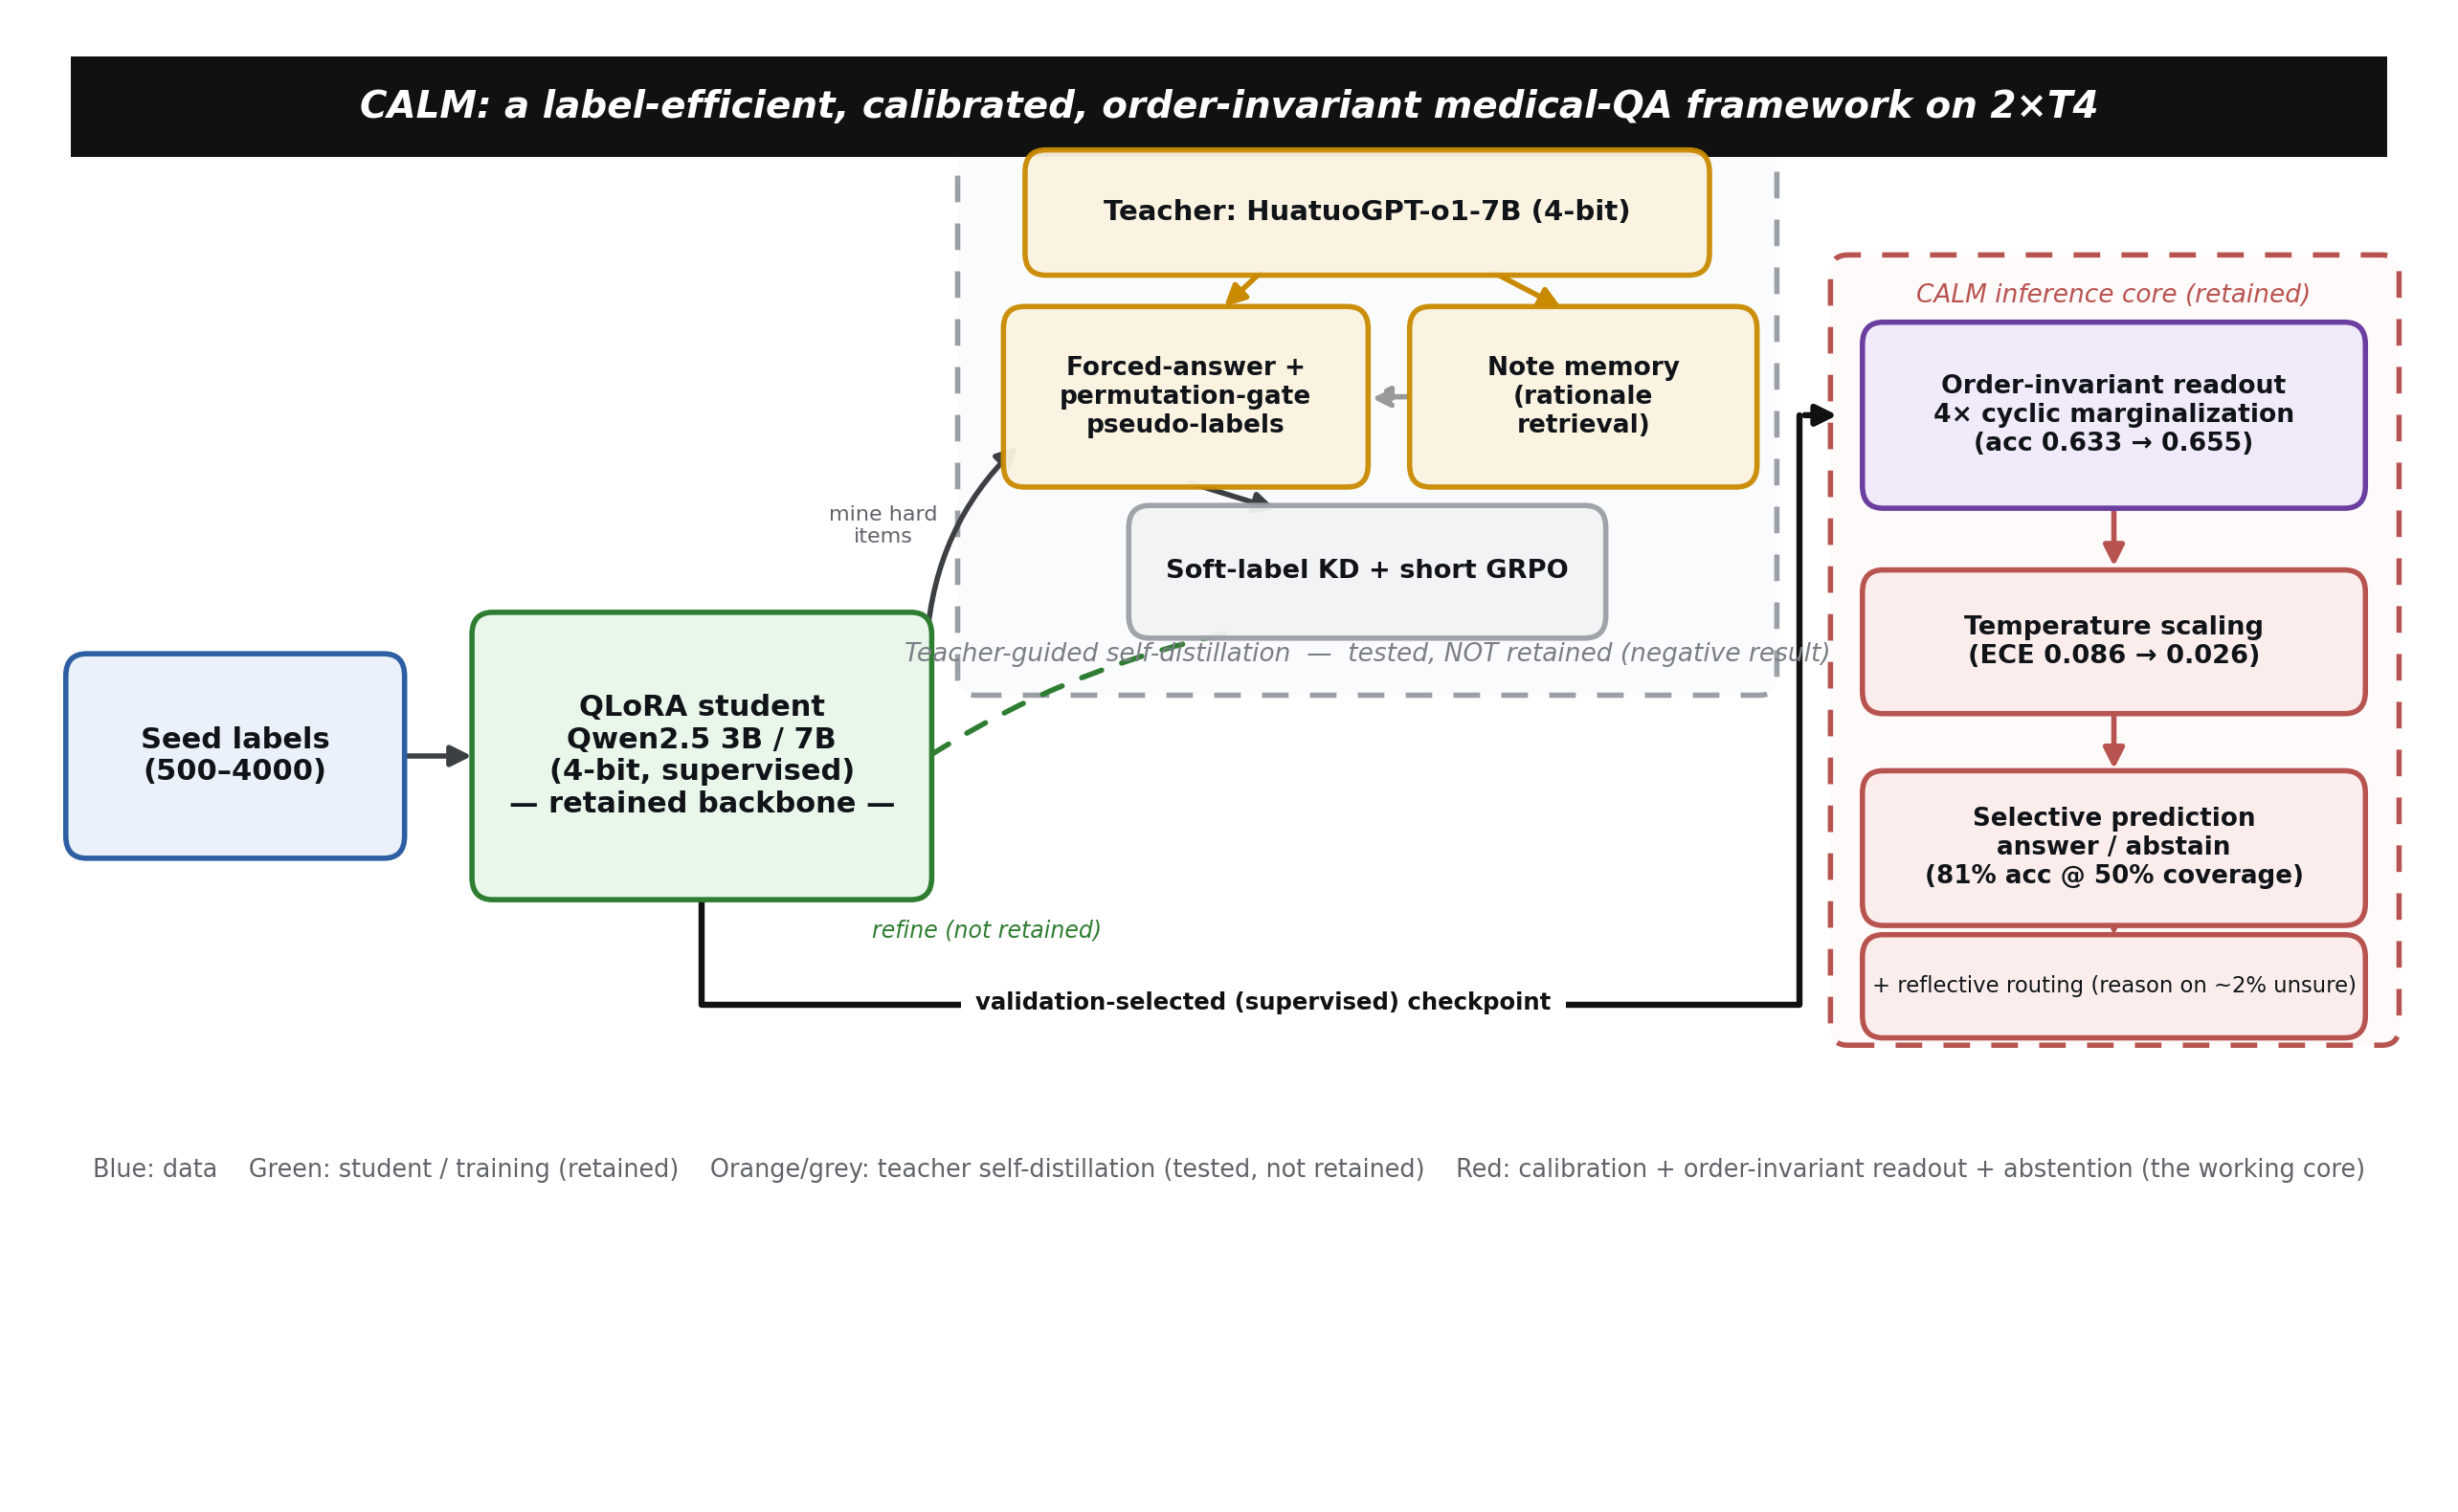
\includegraphics[width=0.95\textwidth]{architecture.png}
\caption{The CALM framework. A QLoRA student is supervised on a small seed set, optionally refined by a teacher-guided self-distillation stage, and equipped with a post-hoc calibration-and-abstention layer. Our ablations show the calibration-and-abstention layer delivers the practical value at this budget, while the self-distillation stage does not improve validation accuracy and is therefore not retained by the checkpoint rule.}
\label{fig:arch}
\end{figure*}

\subsection{Setup and student}
Each item has a stem $x$, four options, and a gold letter $y\in\{A,B,C,D\}$. We draw a seed set $\mathcal{D}_{\text{seed}}$ of 500 to 4{,}000 labeled items and treat the remaining train split as an unlabeled pool $\mathcal{U}$. The student is Qwen2.5-3B-Instruct or Qwen2.5-7B-Instruct \cite{qwen}, loaded in 4-bit NF4 and adapted with LoRA on the attention and MLP projections \cite{lora,qlora}. We score an answer from the next-token logits at the answer position. Each option letter $k$ has a small set $V_k$ of clean single-token encodings (bare and leading-space forms); we aggregate their logits as $\ell_k=\log\sum_{v\in V_k}\exp z_v$ and normalize,
\begin{equation}
p_\theta(k\mid x)=\frac{\exp \ell_k}{\sum_{j\in\{A,B,C,D\}}\exp \ell_j},
\end{equation}
and train with cross-entropy on $\mathcal{D}_{\text{seed}}$. Logits are read with no intervening reasoning prompt. The selected 7B configuration uses a single epoch; the 3B headline run used two epochs and became overconfident (Section~\ref{sec:results}), so longer schedules were not retained for the 7B model.

\subsection{Difficulty mining}
We rank $\mathcal{U}$ by a score that prefers uncertain items,
\begin{equation}
s(x)=\alpha\,\tilde{H}(x)+(1-\alpha)\bigl(1-\textstyle\max_k p_\theta(k\mid x)\bigr)+\beta\,(1-m(x)),
\end{equation}
where $\tilde{H}(x)$ is the (unnormalized) option-distribution entropy, with range $[0,\log 4]$, $m(x)=p_{(1)}(x)-p_{(2)}(x)$ is the top-two probability margin, and $\alpha=0.5$, $\beta=0.3$ are weights on this unnormalized scale. The highest-scoring items are sent to the teacher.

\subsection{Pseudo-labeling with two agreement gates}
A teacher label is kept only if it passes two checks. \emph{Permutation consistency}: the teacher is queried on the original option order and on a random permutation, and the selected option must match after re-indexing. \emph{Teacher confidence}: the teacher's maximum option probability---its first-token softmax over the same four letter ids, taken from a direct answer rather than parsed from generated text---must exceed $\gamma=0.55$. Survivors form $\mathcal{P}$ with the teacher distribution $p_T$ (the parsed option softmax) as a soft target. We audit, but never train on, the oracle accuracy of these pseudo-labels.

\subsection{Note memory, synthesis, and contamination screen}
For accepted items the teacher writes a one- or two-sentence rationale, embedded with all-MiniLM-L6-v2 and stored for nearest-neighbor retrieval; near-duplicates (cosine $\ge 0.92$) are dropped. For a subset of hard items the teacher rewrites the stem to create neighbors, admitted only when a verifier re-derives the same answer (synthetic near-duplicates with cosine $\ge 0.95$ are removed). As a fixed, pre-specified contamination audit, every synthetic and pseudo item is compared by embedding cosine to the test questions and discarded above $0.95$; this screen uses no labels and no outcome feedback. Because $\mathcal{U}$ is drawn from the training split, the screen removed zero items in both reported runs, but we keep it as a guard.

\subsection{Distillation and reinforcement}
We mix seed cross-entropy with a confidence-weighted distillation term over $\mathcal{P}$. Let $p_\theta^{(T)}(k\mid x)\propto\exp(\ell_k/T_{\text{KD}})$ be the temperature-softened student distribution. The teacher provides parsed option probabilities $p_T$ (not logits), softened as $p_T^{(T)}(k\mid x)=p_T(k\mid x)^{1/T_{\text{KD}}}\big/\sum_j p_T(j\mid x)^{1/T_{\text{KD}}}$. Then
\begin{equation}
\mathcal{L}=\mathbb{E}_{x\sim\mathcal{D}_{\text{seed}}}\!\big[\mathcal{L}_{\text{CE}}\big]
+\lambda\,T_{\text{KD}}^{2}\,\mathbb{E}_{x\sim\mathcal{P}}\!\big[w(x)\,\mathrm{KL}\!\big(p_T^{(T)}\Vert p_\theta^{(T)}\big)\big],
\end{equation}
with distillation temperature $T_{\text{KD}}=3$, weight $\lambda=0.5$, and per-example weight $w(x)$ the teacher's confidence; the $T_{\text{KD}}^2$ factor restores the gradient scale of the softened targets. A short group-relative pass \cite{grpo} then rewards the student for matching accepted labels, anchored by a KL term to a frozen reference obtained by disabling the LoRA adapter.

\subsection{Calibration and selective prediction}
After training we fit a single calibration temperature $T_{\text{cal}}$ on the validation logits by minimizing NLL \cite{guocal}, distinct from the distillation $T_{\text{KD}}$. Confidence is the maximum post-$T_{\text{cal}}$ softmax probability. We report expected calibration error with ten equal-width bins,
\begin{equation}
\mathrm{ECE}=\sum_{b=1}^{10}\frac{|S_b|}{n}\,\bigl|\,\mathrm{acc}(S_b)-\mathrm{conf}(S_b)\,\bigr|,
\end{equation}
the multiclass Brier score $\frac{1}{n}\sum_i\sum_k (p_{ik}-\mathbf{1}[y_i=k])^2$, and NLL. For abstention we rank predictions by confidence; at coverage $\tau$ the system answers the top fraction $\tau$, with risk $r(\tau)=1-\mathrm{acc}(\tau)$, and we summarize by $\mathrm{AURC}=\int_0^1 r(\tau)\,d\tau$ (trapezoidal over the test set). ``Coverage at 80\% accuracy'' is the largest $\tau$ whose answered accuracy stays at or above $0.80$. These risk--coverage quantities are computed on the test split from the calibrated-confidence ranking; they characterize that ordering and are not thresholds tuned on test labels. We did not select any operating threshold using the test set.

\subsection{Checkpoint selection}
\label{sec:selection}
All checkpoints are selected on the \emph{validation} split, never on test. We keep the model with the best validation accuracy. Test metrics are then reported for the selected checkpoint, together with diagnostic analyses (the label-efficiency points, the ablation, the readout comparisons, and the shuffle and contamination checks) that we mark as post-selection rather than as model selection. As Section~\ref{sec:results} shows, the self-distilled checkpoint had lower validation accuracy than the supervised one for both students, so the rule retains the supervised model.

\section{Experimental Setup}
Each run was constrained to one Kaggle session with two Tesla T4 GPUs (16\,GB each); the student occupies one card and the 4-bit teacher the other. The data are MedQA-USMLE four-option multiple-choice questions; we use a fixed 1{,}000-item validation split and a 1{,}273-item test split. Training uses AdamW with a cosine schedule, gradient checkpointing, and last-token logits only to stay in budget, and a wall-clock guard stops gracefully before the 12-hour session limit. Table~\ref{tab:impl} lists the hyperparameters for both runs. We report accuracy, macro-F1, ECE, Brier, NLL, 95\% bootstrap intervals (2{,}000 resamples), an option-order shuffle check, and the abstention metrics above. For the readout and routing comparisons we additionally report \emph{paired} bootstrap intervals on the per-item accuracy difference, which test whether a method beats the base reader on the same items. No out-of-memory event occurred on either 16\,GB card.

\begin{table}[tb]
\caption{Implementation details for the two reported runs. The cosine row lists thresholds for the test-question screen, note de-duplication, and synthetic de-duplication, respectively.}
\label{tab:impl}
\centering
\footnotesize
\setlength{\tabcolsep}{4pt}
\begin{tabular}{@{}lcc@{}}
\toprule
Setting & 3B run & 7B run \\
\midrule
Student & Qwen2.5-3B-Instruct & Qwen2.5-7B-Instruct \\
Quantization & 4-bit NF4 & 4-bit NF4 \\
LoRA rank / $\alpha$ / dropout & 32 / 64 / 0.05 & 16 / 32 / 0.05 \\
LoRA targets & \multicolumn{2}{c}{q,k,v,o,gate,up,down} \\
Seed labels (headline) & 4000 & 2000 \\
SFT epochs / LR & 2 / $1.5\!\times\!10^{-4}$ & 1 / $1\!\times\!10^{-4}$ \\
Batch / grad-accum & 8 / 4 & 4 / 8 \\
Max source length & 512 & 448 \\
Teacher & \multicolumn{2}{c}{HuatuoGPT-o1-7B (4-bit)} \\
Mining $\alpha,\beta$ & \multicolumn{2}{c}{0.5, 0.3} \\
Pseudo gate $\gamma$ & \multicolumn{2}{c}{0.55} \\
Decontam./note/synth cos. & \multicolumn{2}{c}{0.95 / 0.92 / 0.95} \\
KD $T_{\text{KD}},\lambda$, epochs & \multicolumn{2}{c}{3.0, 0.5, 2} \\
GRPO group / LR / KL / epochs & \multicolumn{2}{c}{6 / $5\!\times\!10^{-6}$ / 0.1 / 1} \\
Embedder & \multicolumn{2}{c}{all-MiniLM-L6-v2} \\
ECE bins & \multicolumn{2}{c}{10 (equal width)} \\
\bottomrule
\end{tabular}
\end{table}

\section{Results}
\label{sec:results}

\subsection{Headline numbers}
Table~\ref{tab:main} reports both students. The 7B model answers 63.3\% of the test set, up from a 59.2\% zero-shot baseline, and the calibration gain is larger than the accuracy gain: raw ECE falls from 0.086 to 0.026 after temperature scaling ($T_{\text{cal}}=1.32$). The 3B model reaches 52.0\%; trained for two epochs it became overconfident (raw ECE 0.36, needing $T_{\text{cal}}=3.6$), whereas one epoch on the 7B model avoided that. The 7B headline has a 95\% bootstrap accuracy interval of [0.606, 0.660] and macro-F1 interval [0.604, 0.657]; accuracy under a random option-order shuffle is 0.631. Calibrated Brier and NLL are 0.48 and 0.89.

\begin{table}[tb]
\caption{Main results on the MedQA-USMLE test split (1{,}273 items). Final = validation-selected checkpoint (Section~\ref{sec:selection}).}
\label{tab:main}
\centering
\small
\setlength{\tabcolsep}{3.5pt}
\begin{tabular}{@{}lcccccc@{}}
\toprule
Student & Labels & Zero-shot & Final acc & F1 & ECE$_\text{raw}$ & ECE$_\text{cal}$ \\
\midrule
Qwen2.5-3B & 4000 & 0.481 & 0.520 & 0.517 & 0.356 & 0.046 \\
Qwen2.5-7B & 2000 & 0.592 & \textbf{0.633} & \textbf{0.631} & 0.086 & \textbf{0.026} \\
\bottomrule
\end{tabular}
\end{table}

\subsection{Label efficiency and model scale}
Table~\ref{tab:eff} sweeps the seed size; each point is a single run, so we read them as observations from this sweep rather than as a general law. The 7B curve rises then flattens: 500 labels give 60.1\%, and quadrupling to 2{,}000 adds about three points while calibration stays tight. The 3B curve is lower and non-monotone (0.533, 0.490, 0.522, 0.520), which we attribute to overfitting a small adapter to a small subset, since that run reached near-zero training loss and required a large $T_{\text{cal}}$. The clearest signal sits between the rows. The 7B configuration scores about eleven points above the 3B one, more than label count moves either model. These two configurations also differ in LoRA rank, epochs, and learning rate (Table~\ref{tab:impl}), so the fair reading is that the stronger base, not parameter count by itself, was the larger lever. Over this range a small team gains more from a better base than from extra annotation.

\begin{table}[tb]
\caption{Label-efficiency sweep (test accuracy; single runs). Calibrated ECE in parentheses for 7B.}
\label{tab:eff}
\centering
\small
\begin{tabular}{@{}lcccc@{}}
\toprule
Student & 500 & 1000 & 2000 & 4000 \\
\midrule
Qwen2.5-3B & 0.533 & 0.490 & 0.522 & 0.520 \\
Qwen2.5-7B & 0.601 (0.024) & 0.613 (0.019) & 0.633 (0.026) & --- \\
\bottomrule
\end{tabular}
\end{table}

\subsection{Calibration and abstention}
Figure~\ref{fig:reliability} (left) shows the 7B reliability diagram before and after temperature scaling; the calibrated curve sits near the diagonal, and confidence separates correct from incorrect answers, which an abstention rule exploits. Table~\ref{tab:abstain} and Figure~\ref{fig:reliability} (right) give the deferral behavior: on this test split, at 50\% coverage the 7B model is correct 80.8\% of the time, and it can answer just over half the questions while holding 80\% accuracy. These selective-prediction values are single-split point estimates; per-coverage bootstrap intervals are left to future work. Errors are spread across the four options rather than collapsing to one, consistent with the shuffle check.

\begin{table}[tb]
\caption{Selective prediction on the test split: risk--coverage summaries from the calibrated-confidence ranking (not a threshold tuned on test). acc@$c$ is accuracy on the most-confident $c\%$ of test items; cov@80 is the largest coverage whose answered accuracy stays $\ge$0.80; AURC is the area under the risk--coverage curve (lower is better). Point estimates.}
\label{tab:abstain}
\centering
\small
\setlength{\tabcolsep}{4pt}
\begin{tabular}{@{}lccccc@{}}
\toprule
Student & acc@50 & acc@70 & acc@90 & AURC & cov@80 \\
\midrule
Qwen2.5-3B & 0.668 & 0.608 & 0.548 & 0.321 & 0.144 \\
Qwen2.5-7B & \textbf{0.808} & \textbf{0.737} & \textbf{0.668} & \textbf{0.185} & \textbf{0.513} \\
\bottomrule
\end{tabular}
\end{table}

\begin{figure*}[t]
\centering
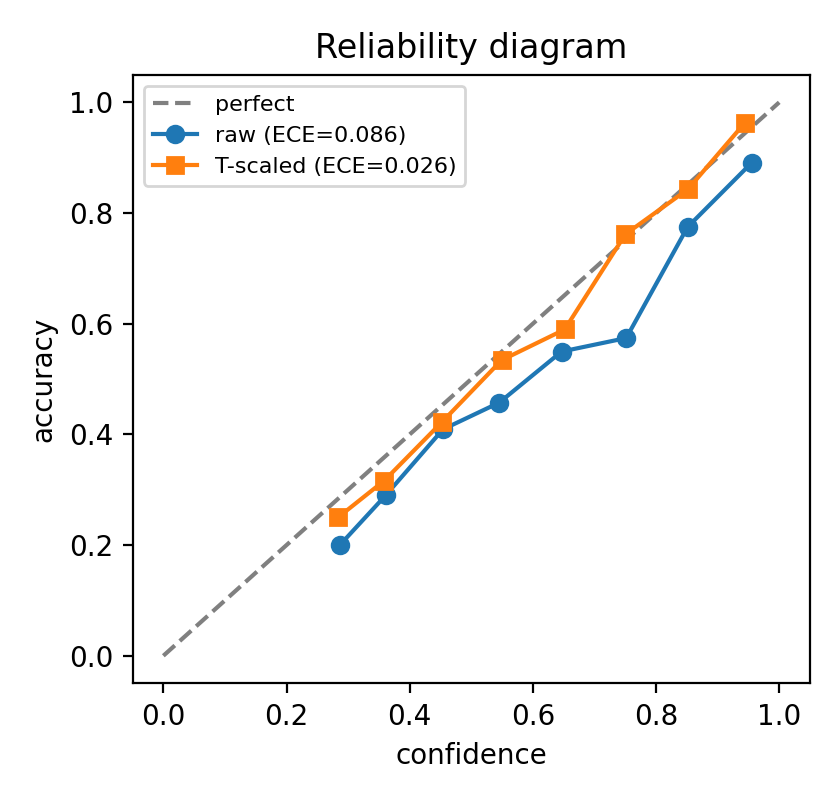
\includegraphics[height=5cm]{reliability_combined.png}\hspace{0.05\textwidth}
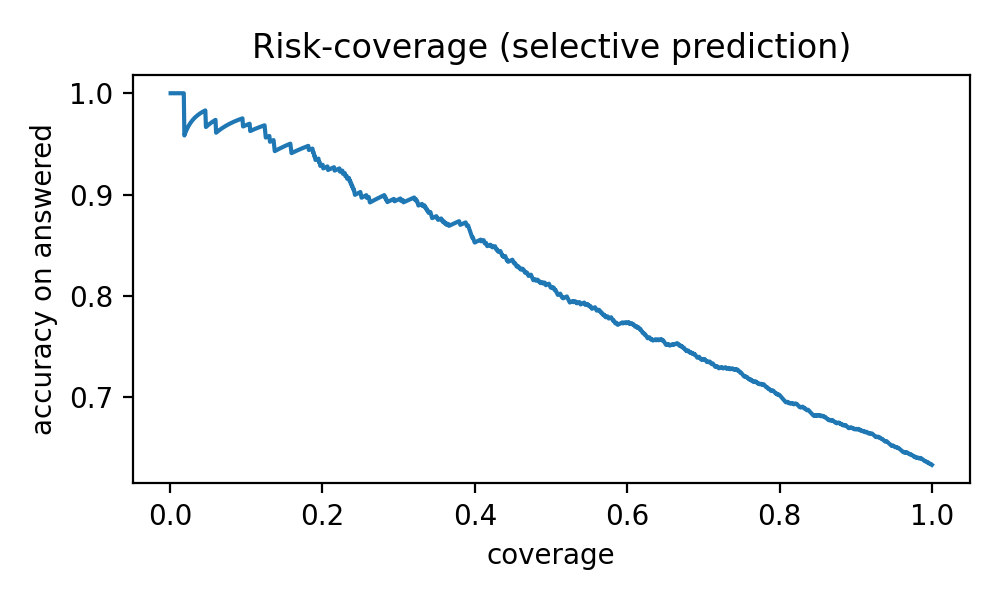
\includegraphics[height=5cm]{risk_coverage.png}
\caption{Calibration and selective prediction for the 7B student. \emph{Left:} reliability diagram before and after temperature scaling (ECE $0.086\!\to\!0.026$); the calibrated curve sits near the diagonal. \emph{Right:} risk--coverage; answering the most confident half raises test accuracy from 63\% to 81\%.}
\label{fig:reliability}
\end{figure*}

\subsection{An order-invariant readout}
\label{sec:pi}
A multiple-choice reader can change its answer when the four options are reordered \cite{robustmcq,permbias}, and our 7B student is mildly sensitive: across the four cyclic orderings its accuracy spans 0.623 to 0.651. We turn that into a fix. For each question we evaluate the four cyclic shifts of the option block, so every option content appears in each letter position exactly once, read the per-content probability from each shift, and average,
\begin{equation}
\bar{p}(c\mid x)=\frac{1}{4}\sum_{s=0}^{3}
p_\theta\!\big(\ell=(c-s)\bmod 4 \;\big|\; x,\pi_s\big),
\end{equation}
where $\pi_s$ is the cyclic shift by $s$ and $\ell$ is the displayed letter. We then apply the same temperature calibration to $\bar{p}$. The readout is training-free and costs four forward passes with no decoding.

Table~\ref{tab:pi} reports the effect on the full test split with paired bootstrap intervals. Marginalization raises accuracy from 0.633 to 0.655---a paired gain of $+0.022$ with 95\% CI $[+0.006,+0.038]$---and improves selective prediction (AURC $0.185\!\to\!0.177$, Brier $0.480\!\to\!0.469$). The marginal accuracy intervals of the base and marginalized readers overlap; the paired interval, which compares the two on the same items, is what establishes the gain. A natural baseline---removing the model's option-ID prior in the style of PriDe \cite{robustmcq}---does nothing here ($+0.000$, CI $[-0.018,+0.018]$): the estimated prior is nearly uniform, $[0.25,0.25,0.26,0.24]$, so there is no letter bias to subtract. The gain is therefore not debiasing but variance reduction: the marginalized reader (0.655) exceeds even the best single ordering (0.651), behaving as a four-way self-ensemble over option placements. Calibration stays tight (ECE 0.032). Figure~\ref{fig:pi} shows the marginalized reader's risk--coverage curve lying below the base curve at every coverage.

\begin{table}[tb]
\caption{Readouts on the full MedQA-USMLE test split (1{,}273 items), all temperature-calibrated. ``passes'' is forward passes per question; none decode tokens. $\Delta$acc is the \emph{paired} accuracy gain over the base reader with 95\% bootstrap CI.}
\label{tab:pi}
\centering
\small
\setlength{\tabcolsep}{3.5pt}
\begin{tabular}{@{}lccccc@{}}
\toprule
Readout & passes & acc & ECE & AURC & $\Delta$acc (95\% CI) \\
\midrule
Base (calibrated)        & 1 & 0.633 & 0.024 & 0.185 & --- \\
PriDe \cite{robustmcq}   & 1 & 0.633 & 0.041 & 0.188 & $+0.000$ $[-0.018,+0.018]$ \\
\textbf{Cyclic-marg.\ (ours)} & 4 & \textbf{0.655} & 0.032 & \textbf{0.177} & $\mathbf{+0.022}$ $[+0.006,+0.038]$ \\
\bottomrule
\end{tabular}
\end{table}

\begin{figure}[tb]
\centering
\includegraphics[width=\linewidth]{pi_risk_coverage.png}
\caption{Risk--coverage on the test split for the base calibrated reader and the order-invariant (cyclic-marginalized) reader. The marginalized curve lies below the base at all coverages (lower risk is better), so the readout improves both accuracy and selective prediction.}
\label{fig:pi}
\end{figure}

\subsection{Selective reasoning and reflective routing}
\label{sec:r3}
Reasoning does not help this student in bulk. On a matched 134-item subset (Table~\ref{tab:sc}) a single calibrated pass beats five-sample self-consistency on both accuracy (0.709 vs 0.493) and selective prediction (AURC 0.128 vs 0.289), at a tiny fraction of the decoding: one forward pass that reads four option logits versus five sampled chains of up to 256 tokens. The likely cause is that fine-tuning the student as a one-shot answerer dulls the chain-of-thought ability the base model had.

That raises a sharper question: does reasoning help \emph{where the model is unsure}? We route on calibrated confidence---answer with the fast logit read when the top option is confident, and otherwise send the question to a single reasoning pass---selecting the confidence threshold on validation. Table~\ref{tab:r3} shows the trade-off on the full test split. Routing only the least-confident $\approx$2\% of items raises accuracy from 0.633 to 0.639, a paired gain of $+0.006$ with 95\% CI $[+0.002,+0.012]$, at roughly two extra decoded tokens per question amortized over the whole split. It is a small but significant adaptive-compute gain, and it comes from \emph{routing alone}: training a dedicated reflect adapter on the hard slice with a reflective-correction objective---cross-entropy toward the gold answer where the fast pass is wrong, consistency with the confident fast prediction where it is right---did not beat the base student's own reasoning ($+0.002$, CI $[-0.002,+0.008]$) and slightly underperformed it, consistent with overfitting a few hundred hard examples. Where reasoning is spent matters more than specializing a separate module.

\begin{table}[tb]
\caption{Reflective routing on the full test split. $\Delta$acc is the \emph{paired} gain over the fast-only reader with 95\% bootstrap CI; tokens/q is decoded tokens per question amortized over the split.}
\label{tab:r3}
\centering
\small
\setlength{\tabcolsep}{3pt}
\begin{tabular}{@{}lcccc@{}}
\toprule
Policy & acc & $\Delta$acc (95\% CI) & \% reasoned & tokens/q \\
\midrule
Fast-only & 0.633 & --- & 0 & 0 \\
\textbf{Routed (untrained reason.)} & \textbf{0.639} & $\mathbf{+0.006}$ $[+0.002,+0.012]$ & 2 & 2.2 \\
Routed (trained reflect adapter) & 0.636 & $+0.002$ $[-0.002,+0.008]$ & 2 & 2.0 \\
\bottomrule
\end{tabular}
\end{table}

\begin{table}[tb]
\caption{Single calibrated pass vs.\ self-consistency reasoning (7B, matched 134-item subset).}
\label{tab:sc}
\centering
\small
\setlength{\tabcolsep}{4pt}
\begin{tabular}{@{}lccc@{}}
\toprule
Method & Acc & AURC & samples $\times$ gen.\ tokens \\
\midrule
Single calibrated pass & \textbf{0.709} & \textbf{0.128} & $1\times1$ (logit read) \\
Self-consistency CoT & 0.493 & 0.289 & $5\times{\le}256$ \\
\bottomrule
\end{tabular}
\end{table}

\subsection{Design analysis: the self-distillation stage}
Table~\ref{tab:abl} contrasts supervised adaptation with the full teacher-guided stage. For both students the stage lowered \emph{validation} accuracy---7B from 0.637 to 0.614, 3B from 0.514 to 0.507---and test accuracy moved the same way (7B 0.633$\to$0.614; 3B 0.520$\to$0.517). The validation-based rule of Section~\ref{sec:selection} therefore keeps the supervised checkpoint, and the headline numbers are those of the supervised model. The cause is visible in the logs: the teacher accepts only a few dozen labels on the hard items, at oracle accuracy near 0.46--0.66, against thousands of clean seed labels---too few, too noisy, and concentrated where teacher and student are both unsure. We report this as a negative result: at this budget, the self-distillation stage of CALM is not the component that helps. The pipeline audit (Table~\ref{tab:audit}) shows the scale: for the 7B run the gates reduced 150 mined items to 79 permutation-consistent and 68 after the confidence gate, 80 synthetic items were kept and 35 rejected, and the test-question screen removed none.

\begin{table}[tb]
\caption{Self-distillation ablation. Validation accuracy decides selection; test accuracy is shown for reference. The stage is not retained.}
\label{tab:abl}
\centering
\small
\setlength{\tabcolsep}{3.5pt}
\begin{tabular}{@{}lcccc@{}}
\toprule
 & \multicolumn{2}{c}{Val acc} & \multicolumn{2}{c}{Test acc} \\
Student & SFT & +self-dist. & SFT & +self-dist. \\
\midrule
Qwen2.5-3B & \textbf{0.514} & 0.507 & 0.520 & 0.517 \\
Qwen2.5-7B & \textbf{0.637} & 0.614 & 0.633 & 0.614 \\
\bottomrule
\end{tabular}
\end{table}

\begin{table}[tb]
\caption{Pseudo-labeling and synthesis audit (one iteration). ``mined'' = items sent to the teacher; ``accepted'' = pseudo-labels passing the permutation and confidence gates; ``oracle PAcc'' = accuracy of accepted pseudo-labels against gold; ``synth.\ kept/rej.'' = synthetic items kept / rejected; ``decon.'' = items removed by the test-question screen. ``---'' marks counts not logged for the 3B run.}
\label{tab:audit}
\centering
\small
\setlength{\tabcolsep}{4pt}
\begin{tabular}{@{}lcccccc@{}}
\toprule
Run & mined & accepted & oracle PAcc & synth. kept & synth. rej. & decon. \\
\midrule
3B (4000) & 150 & 79 & 0.658 & --- & --- & 0 \\
7B (2000) & 150 & 68 & 0.456 & 80 & 35 & 0 \\
\bottomrule
\end{tabular}
\end{table}

\subsection{Context}
Table~\ref{tab:context} places our numbers beside larger systems. The values are copied from the cited papers under their own settings and are not directly comparable; we include them only to mark the operating regime. A 7B model fine-tuned from 2{,}000 labels on two free T4s reaches a useful accuracy and, unlike the bare base, comes with calibrated confidence, a working abstention rule, and an order-invariant readout.

\begin{table}[tb]
\caption{Context only. Values are as reported (rounded) by the cited sources under their own settings and are not directly comparable. The Qwen2.5-7B row is the zero-shot value reported by~\cite{qwen}; under our own prompt and evaluation the same base scores 0.592 (Table~\ref{tab:main}).}
\label{tab:context}
\centering
\small
\setlength{\tabcolsep}{3pt}
\begin{tabular}{@{}lccc@{}}
\toprule
System & Size & MedQA & Setting \\
\midrule
GPT-4 \cite{gpt4med} & undisclosed & $\approx$0.86 & prompting \\
Med-PaLM 2 \cite{medpalm} & undisclosed & $\approx$0.86 & full-data \\
Meerkat \cite{meerkat} & 7B & 0.77 & reasoning-data \\
MedMobile \cite{medmobile} & 3.8B & 0.76 & full-data \\
Qwen2.5-7B \cite{qwen} & 7B & $\approx$0.51 & zero-shot \\
\textbf{Ours (7B, 2k labels)} & 7B & \textbf{0.655} & this work \\
\bottomrule
\end{tabular}
\end{table}

\section{Discussion}
A few things stand out. The largest lever in our sweep was the base configuration: the 7B run beat the 3B run by more than label count ever moved either one, and once the base was fixed, a few hundred labels already reached a near-flat region. (The two runs differ in more than parameter count, so we do not claim to isolate scale.) Calibration came next: a single temperature turned an over-sharp classifier into one whose confidence means something, and that confidence drives both abstention and routing. The cheapest accuracy we found came from neither labels nor reasoning but from \emph{symmetry}---averaging over option orderings recovered more than two points for free, and did so by reducing variance rather than removing a bias. Reasoning, by contrast, helped only when spent selectively and sparingly, and a trained reasoning adapter did not help at all. Two further additions we expected to help did not: the self-distillation stage lowered validation accuracy, and self-consistency lost to a single calibrated pass.

Those measurements are what let CALM stay lean. The configuration our validation rule selects is supervised adaptation with calibration, abstention, and an order-invariant readout; the teacher-guided stage and the trained reasoning adapter are kept only as tested options. For small medical-QA models on commodity hardware, that is the recommendation we are willing to defend.

\section{Limitations}
We evaluate on one English benchmark and a single test split, with single-run sweeps rather than multi-seed averages, so the trends should not be read as laws. Accuracy ($\approx$0.65) is well below specialist systems trained on full data. The order-invariant readout costs four forward passes per question (still no decoding), and the routing gain, though significant, is small and rests on a few percent of items. Calibration and abstention are measured post-hoc on a benchmark split; they do not establish robustness under distribution shift, prospective calibration, or any clinical-workflow validation, and we make no deployment claim. The contamination screen against test questions is a fixed, label-free audit, but using test inputs at all is a sensitivity worth noting. The self-consistency cost comparison is a decoding-step argument, not a wall-clock benchmark.

\section{Conclusion}
Two free T4s, a few thousand labels, quantized adapters. On that budget a Qwen2.5-7B QLoRA student reaches 0.633 on the MedQA-USMLE test split and calibrates to an ECE of 0.026 with one parameter; its most confident half answers at 80\% accuracy. A training-free order-invariant readout then lifts accuracy to 0.655 and improves selective prediction, and confidence-gated routing adds a small further gain at negligible compute. We have tried to be plain about what carried the result and what did not: the stronger base, calibration, and order averaging helped; a teacher-guided self-distillation stage, self-consistency, and a trained reflect adapter did not. What is left is a short recipe---stronger base, light supervised adaptation, temperature calibration, abstention, and an order-invariant readout---and a reproducible baseline for medical QA under tight compute.

\section*{Reproducibility}
Training and evaluation code, configuration files, prompts, split definitions, and the exported metric artifacts and figures will be released upon publication so that the reported numbers can be regenerated on the same two-T4 setup.

\section*{Acknowledgment}
The authors thank the open-source community and Kaggle for accessible T4 compute. A generative AI assistant was used for grammar and copy-editing of the manuscript; all experimental design, code, analysis, and conclusions are the authors' own, and the authors take full responsibility for the content.

\begin{thebibliography}{00}
\bibitem{medqa} D. Jin, E. Pan, N. Oufattole, W.-H. Weng, H. Fang, and P. Szolovits, ``What disease does this patient have? A large-scale open domain question answering dataset from medical exams,'' \emph{Applied Sciences}, vol.~11, no.~14, 2021.
\bibitem{gpt4med} H. Nori, N. King, S. M. McKinney, D. Carignan, and E. Horvitz, ``Capabilities of GPT-4 on medical challenge problems,'' arXiv:2303.13375, 2023.
\bibitem{medpalm} K. Singhal \emph{et al.}, ``Towards expert-level medical question answering with large language models,'' \emph{Nature Medicine}, 2025.
\bibitem{meerkat} H. Kim \emph{et al.}, ``Small language models learn enhanced reasoning skills from medical textbooks,'' \emph{npj Digital Medicine}, 2025.
\bibitem{medmobile} K. Vishwanath \emph{et al.}, ``MedMobile: A mobile-sized language model with clinical capabilities,'' arXiv:2410.09019, 2024.
\bibitem{huatuo} J. Chen \emph{et al.}, ``HuatuoGPT-o1: Towards medical complex reasoning with LLMs,'' arXiv:2412.18925, 2024.
\bibitem{hinton} G. Hinton, O. Vinyals, and J. Dean, ``Distilling the knowledge in a neural network,'' arXiv:1503.02531, 2015.
\bibitem{star} E. Zelikman, Y. Wu, J. Mu, and N. Goodman, ``STaR: Bootstrapping reasoning with reasoning,'' in \emph{NeurIPS}, 2022.
\bibitem{selfconsistency} X. Wang \emph{et al.}, ``Self-consistency improves chain of thought reasoning in language models,'' in \emph{ICLR}, 2023.
\bibitem{pseudolabel} D.-H. Lee, ``Pseudo-label: The simple and efficient semi-supervised learning method for deep neural networks,'' in \emph{ICML Workshop}, 2013.
\bibitem{lora} E. J. Hu \emph{et al.}, ``LoRA: Low-rank adaptation of large language models,'' in \emph{ICLR}, 2022.
\bibitem{qlora} T. Dettmers, A. Pagnoni, A. Holtzman, and L. Zettlemoyer, ``QLoRA: Efficient finetuning of quantized LLMs,'' in \emph{NeurIPS}, 2023.
\bibitem{guocal} C. Guo, G. Pleiss, Y. Sun, and K. Q. Weinberger, ``On calibration of modern neural networks,'' in \emph{ICML}, 2017.
\bibitem{selectivenet} Y. Geifman and R. El-Yaniv, ``SelectiveNet: A deep neural network with an integrated reject option,'' in \emph{ICML}, 2019.
\bibitem{abstain} H. Wen \emph{et al.}, ``Know your limits: A survey of abstention in large language models,'' \emph{Transactions of the Association for Computational Linguistics}, 2025.
\bibitem{trustsurvey} Y. Wang, R. E. Mercer, F. Rudzicz \emph{et al.}, ``Trustworthy medical question answering: An evaluation-centric survey,'' arXiv:2506.03659, 2025.
\bibitem{robustmcq} C. Zheng, H. Zhou, F. Meng, J. Zhou, and M. Huang, ``Large language models are not robust multiple choice selectors,'' in \emph{Proc. ICLR}, 2024.
\bibitem{permbias} Y. Zong, T. Yu, R. Chavhan, B. Zhao, and T. Hospedales, ``Fool your (vision and) language model with embarrassingly simple permutations,'' in \emph{Proc. ICML}, 2024.
\bibitem{grpo} Z. Shao \emph{et al.}, ``DeepSeekMath: Pushing the limits of mathematical reasoning in open language models,'' arXiv:2402.03300, 2024.
\bibitem{smallrl} Q. Dao \emph{et al.}, ``Reinforcement learning for reasoning in small LLMs: What works and what doesn't,'' arXiv:2503.16219, 2025.
\bibitem{qwen} A. Yang \emph{et al.}, ``Qwen2.5 technical report,'' arXiv:2412.15115, 2024.
\end{thebibliography}

\end{document}
